% !TEX TS-program = pdflatex
% !TEX encoding = UTF-8 Unicode

\documentclass{beamer}
\usepackage[czech]{babel}
\usepackage[utf8]{inputenc}
\usepackage{times}
\usepackage[T1]{fontenc}
\usepackage{verbatim}
\usepackage{listings}
\usepackage{xcolor}

\mode<presentation>
{
	\usetheme{antibes}
	\usecolortheme{orchid}
}

\setbeamertemplate{navigation symbols}{}

\definecolor{cmtgreen}{RGB}{0,192,0}

\begin{document}

\title{C++; delete Java;}
\subtitle{Část 6: smart pointery}
\author{Kennny}
\date{srpen 2017}

\frame{\titlepage}

\lstset{language=C++,
        basicstyle=\ttfamily,
        keywordstyle=\color{blue}\ttfamily,
        stringstyle=\color{red}\ttfamily,
        commentstyle=\color{cmtgreen}\ttfamily,
        morecomment=[l][\color{magenta}]{\#}
}

\newenvironment{xframe}[1][]
  {\begin{frame}[fragile,environment=xframe,#1]}
  {\end{frame}}

\begin{comment}
\begin{xframe}{tttt}
	\begin{itemize}
		\item
	\end{itemize}
\end{xframe}
\end{comment}



\section{Smart pointery}
\subsection{Obecné}

\begin{xframe}{Motivace}
	\begin{itemize}
		\item eliminovat memory leaky
		\item pracovat s pamětí bezpečně
		\item využít moderní principy OOP
		\item vyhnout se garbage collectoru
	\end{itemize}
	\begin{quote}
\uv{If Java had true garbage collection, most programs would delete themselves upon execution.}
		\end{quote}
\end{xframe}

\begin{xframe}{Řešení}
	\begin{itemize}
		\item smart pointery
		\item v zásadě existují tři (šablonové) typy:
			\begin{itemize}
				\item \texttt{unique\_ptr}
				\item \texttt{shared\_ptr}
				\item \texttt{weak\_ptr}
			\end{itemize}
		\item dříve ještě \texttt{auto\_ptr}, nyní deprecated
	\end{itemize}
\end{xframe}

\begin{xframe}{Smart pointery}
	\begin{itemize}
		\item reference counting
		\item RAII struktury
			\begin{itemize}
				\item konstruktor zvyšuje čítač
				\item destruktor snižuje
			\end{itemize}
		\item podporují vlastnosti OOP (dědičnost, polymorfismus, ..)
	\end{itemize}
\end{xframe}

\subsection{Konkrétní typy}

\begin{xframe}{std::unique\_ptr}
	\begin{itemize}
		\item unikátní ukazatel - ve smyslu vlastníka
		\item takový objekt má pouze jednoho vlastníka
		\item nedá se kopírovat, pouze přesunout (zneplatní původní)
		\item přetížen operátor \texttt{->} pro přístup k paměti, aby se choval jako každý jiný pointer
		\item lze vyzvednout surový pointer metodou \texttt{get()}
		\item vytváření pomocí \texttt{std::make\_unique} s parametry konstruktoru
\begin{lstlisting}[basicstyle=\fontsize{8}{9}\selectfont\ttfamily]
std::unique_ptr<Coords> a = std::make_unique<Coords>(5.5, 2.5);
// analogie k puvodnimu
Coords* b = new Coords(5.5 2.5);
\end{lstlisting}
	\end{itemize}
\end{xframe}

\begin{xframe}{Příklad}
	\begin{itemize}
		\item Prostor pro příklad 06\_a\_unique\_ptr
	\end{itemize}
\end{xframe}

\begin{xframe}{std::shared\_ptr}
	\begin{itemize}
		\item "silný"~ukazatel
		\item reference counting v plné podobě
		\item také přetížen operátor \texttt{->}
		\item lze vyzvednout surový pointer metodou \texttt{get()}
		\item vytváření pomocí \texttt{std::make\_shared} s parametry konstruktoru
\begin{lstlisting}[basicstyle=\fontsize{8}{9}\selectfont\ttfamily]
std::shared_ptr<Coords> a = std::make_shared<Coords>(5.5, 2.5);
// analogie k puvodnimu
Coords* b = new Coords(5.5 2.5);
\end{lstlisting}
	\end{itemize}
\end{xframe}

\begin{xframe}{std::shared\_ptr}
	\begin{itemize}
		\item již lze kopírovat
\begin{lstlisting}[basicstyle=\fontsize{8}{9}\selectfont\ttfamily]
std::shared_ptr<Coords> a = std::make_shared<Coords>(5.5, 2.5);
std::shared_ptr<Coords> b = a;
std::shared_ptr<Coords> c = b;
\end{lstlisting}
		\item všechny ukazují na stejné místo, reference counter je roven 3
		\item jakmile se zavolají destruktory, sníží se counter na 0 a poslední destruktor ho dealokuje
		\item asi nejběžnější varianta smart pointeru
	\end{itemize}
\end{xframe}

\begin{xframe}{Příklad}
	\begin{itemize}
		\item Prostor pro příklad 06\_a\_shared\_ptr
	\end{itemize}
\end{xframe}

\begin{xframe}{std::weak\_ptr}
	\begin{itemize}
		\item "slabý"~ukazatel, který se nepodílí na reference countingu
		\item sdružený se shared pointerem
		\item \alert{nemá} přetížen operátor \texttt{->}
		\item inicializuje se přiřazením shared pointeru
		\item před použitím nutno konvertovat na shared pointer
\begin{lstlisting}[basicstyle=\fontsize{8}{9}\selectfont\ttfamily]
std::weak_ptr<Coords> a = sharedPtrCoords;

if (std::shared_ptr<Coords> sptr = a.lock())
    sptr->DoSomething();
\end{lstlisting}
		\item pokud již byla paměť smazána, \texttt{lock()} vrátí \texttt{nullptr}
		\item hodí se pro implementaci kruhových závislostí
	\end{itemize}
\end{xframe}

\begin{xframe}{std::weak\_ptr}
	\begin{figure}
		\centering
		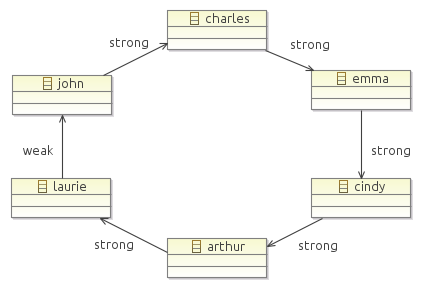
\includegraphics[width=0.75\textwidth]{sharedweakcircle.png}
		\caption{Kruhová závislost, ukradeno z \url{https://visualstudiomagazine.com/articles/2012/10/19/circular-references.aspx}}
	\end{figure}
\end{xframe}

\begin{xframe}{Příklad}
	\begin{itemize}
		\item Prostor pro příklad 06\_a\_weak\_ptr
	\end{itemize}
\end{xframe}




\begin{xframe}{Konec 6. části}
\texttt{exit(0);}
\end{xframe}




\end{document}




